\documentclass{article}

\usepackage[utf8]{inputenc}
\usepackage[english,russian]{babel}
\usepackage[T2A]{fontenc}
\usepackage{tabularx}
\usepackage{amsmath,mathrsfs,amssymb}
\usepackage{bbding}
\usepackage{alltt}
\usepackage{epigraph}
\usepackage{verbatim}
\usepackage{soul}
\usepackage{latexsym}
\usepackage{array}
\usepackage{comment}
\usepackage{makeidx}
\usepackage{listings}
\usepackage{indentfirst}
\usepackage{verbatim}
\usepackage{color}
\usepackage{url}
\usepackage{xspace}
\usepackage{hyperref}
\usepackage{stmaryrd}
\usepackage{tikz}
\usetikzlibrary{arrows,decorations.pathreplacing,backgrounds,fit,positioning,shapes,chains,calligraphy,arrows.meta,shapes.arrows,overlay-beamer-styles}
\usepackage{euscript}
\usepackage{mathtools}
\usepackage{graphicx}
\usepackage{euscript}
\usepackage{mathtools}
\usepackage{transparent}
\usepackage{bold-extra}

\newcommand{\sembr}[1]{\llbracket{#1}\rrbracket}
\newcommand{\primi}[1]{\mathbf{#1}}
\newcommand{\Int}[2]{\primi{int}^{\mathcal {#1}}_{\mathcal {#2}}}
\newcommand{\Sem}[2]{\sembr{#1}_{\mathcal {#2}}}

\newcommand{\lama}{$\lambda\kern -.1667em\lower -.5ex\hbox{$a$}\kern -.1000em\lower .2ex\hbox{$\mathcal M$}\kern -.1000em\lower -.5ex\hbox{$a$}$\xspace}
\sloppy

\lstdefinelanguage{cc}{
basicstyle=\ttfamily\small,
keywords={include,int,char,float,double,long,short,void,static,volatile,auto,const,return,if,while,else},
keywordstyle=\rmfamily\bfseries,
sensitive=true,
}

\begin{document}

\section{Programming Languages}

Starting a course on programming languages and compilers it makes sense first to stipulate what programming languages are. In a nutshell, programming languages
are languages for writing computer programs. While looking vacuous, this definition nevertheless discovers an important observation: since programming
languages are \emph{languages}, i.e. \emph{sign systems}, to reason about programming languages we can apply the notions and terminology of \emph{semiotics},
a branch of science dealing with sign systems.

\begin{figure}[h]
  \centering
  \includegraphics[scale=0.5]{images/morris.jpg}
  \caption{Charles William Morris (1901-1979)}
  \label{morris}
\end{figure}

One of the founders of semiotics, Charles William Morris, has identified the following important notions:

\begin{itemize}
\item \emph{Syntax}~--- relations between the signs of sign system themselves.
\item \emph{Semantics}~--- relations between a sign system and objects.
\item \emph{Pragmatics}~--- relations between a sign system and a person.
\end{itemize}

In a narrower context of programming languages syntax denotes the form of program representation, semantics~--- the ``meaning'' of programs, and pragmatics~---
the relation between programming language and developer. In our course we focus mainly on syntax and semantics, putting all pragmatics questions aside.

\section{Syntax}

Similarly to natural languages, the syntax of a programming language can be decomposed into a few levels (lexical structure, grammar, etc.) However,
unlike natural languages, which have been evolving more or less spontaneously, the syntax for a programming language is intelligently designed taking
into account a number of specific requirements; in particular, it is (as a rule) \emph{unabiguous} and allows for efficient analysis.

To illustrate the concept of programming language syntax consider the following simple snippet in \textsc{C}:

\begin{figure}[h]
  \centering
  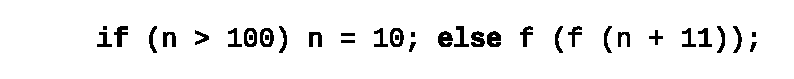
\includegraphics[scale=0.7]{images/01-01.eps}
\end{figure}

From the \emph{lexical} standpoint this fragment can be seen as a sequence of \emph{tokens} (a keyword, a delimiter, an identifier, a binary operator,
a decimal constant, etc.):

\begin{figure}[h]
  \centering
  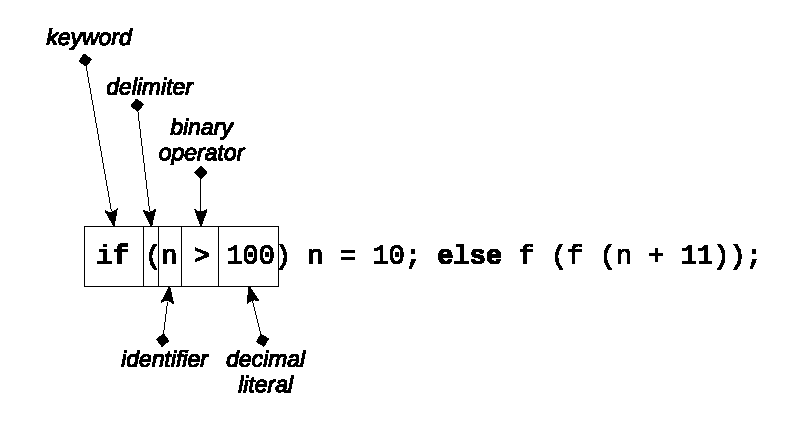
\includegraphics[scale=0.7]{images/01-02.eps}
\end{figure}

This sequence of tokens, in turn, is grouped into an hierarchy of syntactic constructs (in this case, expressions and operators):

\begin{figure}[h]
  \centering
  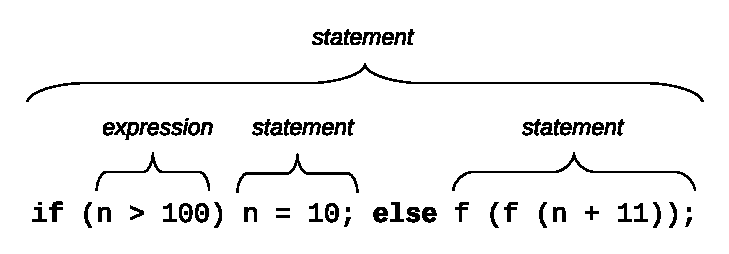
\includegraphics[scale=0.7]{images/01-03.eps}
\end{figure}

Natural languages, as a rule, are \emph{ambiguous}. Consider the following phrase: ``Entering the doors with pets hold them.`` Hold what? The doors or the pets?
In this case we encounter a \emph{global ambiguity} which cannot be resolved even taking into account the context. The only way to resolve it is to
rephrase (``Entering the doors hold your pets'' or ``Hold your pets while entering the doors''). The presence of such unresolvable ambiguities in a
programming language is inacceptable.

\section{Semantics}

The drastic difference between natural and programming languages manifests itself in a full bloom on the semantic level. Unlike natural languages,
for programming languages there are ways to formally specify their semantics and acquire a \emph{mathematically proven} results.

Why formal semantics matters? While in a common practice of using programming languages for application-level software we can rely on our vague, fuzzy
understanding of the meanings of their constructs, when we develop system-level programming \emph{tools}, in particular, compilers, this understanding
turns out to be insufficient. Imagine, for example, that we know that in some programming language expressions consist of variables, constant and four
arithmetic operators. Is this knowledge is complete?

Let us have the following expressions:

\begin{lstlisting}
   0*(x/0)
   1+x-x  
\end{lstlisting}      

What should be the results of their evaluation?

In the first sample, on one hand, the multiplication to zero always gives zero; on the other hand, the division by zero is undefined. So, would the result of
the expression be zero or undefined?

In the second sample, we add a value of \lstinline|x| to \lstinline|1| and immediately subtract it. On one hand this would give us \lstinline|1|; on the
other hand, the value of \lstinline|x| can be undefined, or adding \lstinline|x| to \lstinline|1| might lead to an overflow. So it remains unclear if we
can replace \lstinline|1+x-x| with \lstinline|1| while preserving the behaviour of the program in all cases.

Even if we cannot come up with definite oral answers to these questions we still can write programs using this language; after all, we always can
see what happens in each case if we have a compiler. But what should we do if our task is to implement the \emph{first} compiler for this language?
What happens if we ask a dozen of people to implement a dozen of compilers independently? Whould all these compilers agree in their semantics, or, perhaps, we
eventually will have a dozen of \emph{different} compilers since their authors have \emph{different} intuition? 

One may argue that all these samples come from a very rare and unrealistic use cases. Indeed, how often a new compiler is created, let alone a
dozen of ones? And those snippets with ``murky'' semantics look like antipatterns: why on earth a sane developer whould write ``\lstinline|0*(x/0)|''
instead of ``\lstinline|0|'' or ``\lstinline|1+x-x|'' instead of ``\lstinline|1|''?

The answer, somewhat unexpected, is that actually all these cases are rather \emph{general} then exceptional. Of course, implementing a completely new compiler from scratch is not an
everyday task; however, at the same time programming languages and compilers are rarely developed ``once and for all''. As a rule, both languages
and their compilers evolve through time: new constructs are being added to languages, and new features are being implemented in compilers. Carrying out all of
these routine tasks require a strong semantic foundations. Besides this, compilers by no means are the only semantic-sensitive development instruments:
there is an abundance of other important tools like IDEs, model checkers, static analyzers, debuggers, profilers, etc., all of which have to interpret the
semantics of programs in a coherent way.

Then, not all programs are written directly by human beings. Actually, a fair share of them are generated by other tools, in particular, \emph{preprocessors}
or other \emph{metaprogramming} tools. The results of metaprogramming as a rule look exactly like the samples discussed above: they contain a lot
of vacuous use of constructs and programming language features, and it is \emph{expected} from the underlying compiler to clean up this mess
in a semantics-preserving manner.

Finally, for a compiler there is nothing ``weird'' in those code samples. The reason is simple: compilers do not have intuition. They just 
routinely convert program texts into executables no matter how weird they would look from a human being point of view. To illustrate this,
consider the following short program in \textsc{C}: 

\begin{lstlisting}[language=cc]
m(f,a,s)char*s;
{char c;return f&1?a!=*s++?m(f,a,s):s[11]:f&2?a!=*s++?
1+m(f,a,s):1:f&4?a--?putchar(*s),m(f,a,s):a:f&8?*s?
m(8,32,(c=m(1,*s++,"Arjan Kenter. \no$../.\""),
m(4,m(2,*s++,"POCnWAUvBVxRsoqatKJurgXYyDQbzhLwkNjdMT"
"GeIScHFmpliZEf"),&c),s)):65:(m(8,34,"rgeQjPruaOnDaP"
"eWrAaPnPrCnOrPaPnPjPrCaPrPnPrPaOrvaPndeOrAnOrPnOrPn"
"OaPnPjPaOrPnPrPnPrPtPnPrAaPnBrnnsrnnBaPeOrCnPrOnCaP"
"nOaPnPjPtPnAaPnPrPnPrCaPnBrAnxrAnVePrCnBjPrOnvrCnxr"
"AnxrAnsrOnvjPrOnUrOnornnsrnnorOtCnCjPrCtPnCrnnirWtP"
"nCjPrCaPnOtPrCnErAnOjPrOnvtPnnrCnNrnnRePjPrPtnrUnnr"
"ntPnbtPrAaPnCrnnOrPjPrRtPnCaPrWtCnKtPnOtPrBnCjPronC"
"aPrVtPnOtOnAtnrxaPnCjPrqnnaPrtaOrsaPnCtPjPratPnnaPr"
"AaPnAaPtPnnaPrvaPnnjPrKtPnWaOrWtOnnaPnWaPrCaPnntOjP"
"rrtOnWanrOtPnCaPnBtCjPrYtOnUaOrPnVjPrwtnnxjPrMnBjPr"
"TnUjP"),0);}
main(){return m(0,75,"mIWltouQJGsBniKYvTxODAfbUcFzSp"
"MwNCHEgrdLaPkyVRjXeqZh");}
\end{lstlisting}

If you have any doubts if this is a valid \textsc{C} program, compile and run it. \textsc{C} is never considered as particularly hard to
understand or syntactically challenging (both arguable), yet the program presented is totally incomprehendible. Actually, it
was specifically designed to be such: there is a whole competition in writing \emph{obfuscated}
code\footnote{https://www.cise.ufl.edu/$\tilde\,$manuel/obfuscate/obfuscate.html}. For us, however, the important observation is that this
program no more obfuscated for a compiler as any other one. Our job as compiler implementors is to make them behave is such a way.


\section{The Essence of Translation}

\emph{Translation} is a syntactic transformation of programs in one language into (equivalent) programs into another.
The feasibility of fully automatic translation constituties a drastic difference between programming languages and natural ones.
Although natural language translation techniques and tools made a tremendous progress in a recent years the adequacy of the results
remains the matter of discusstion; and, anyway, this adequacy can not be mathematically proven. For compilers this problem
is essentially solved.

A compiler itself is not a magical creature~--- it is a \emph{program}, written, in turn, in some programming language. Thus, speaking
about compilation, we actually deal with \emph{three} languages:

\begin{figure}[h]
  \centering
  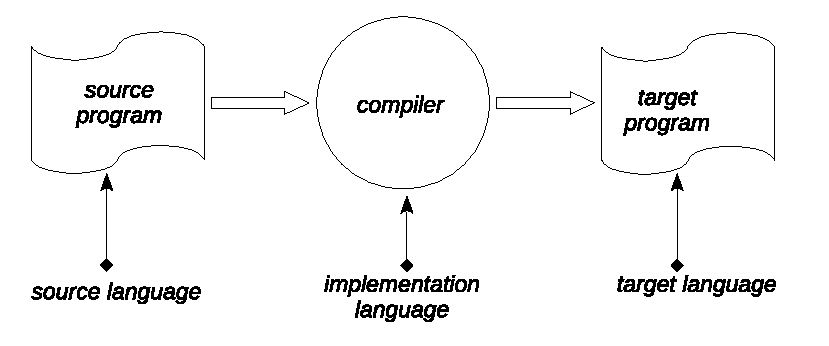
\includegraphics[scale=0.7]{images/01-04.eps}
\end{figure}

\begin{itemize}
\item The language in which the programs being compiled are written (\emph{source language}).
\item The language in which the programs being compiled are compiled (\emph{target language}).
\item The language in which the compiler from source to target language is written (\emph{compiler implementation language}).
\end{itemize}

\section{Translation Subspecies}

As you probably know, there is a subdivision of languages into high- and low-level. This subdivision is not absolute: for example,
\textsc{Haskell} is considered by many as more high-level language than \textsc{C}, which, in turn, is of higher level then \textsc{Fortran}, etc.
As a rule, high-level languages are equipped with type systems, while low-level are not (but \textsc{Scheme} is untyped while there 
exist typed assemblers). This coarse-grained classification of languages leads to a corresponding coarse-grained classification of
translators:

\begin{figure}[h]
  \centering
  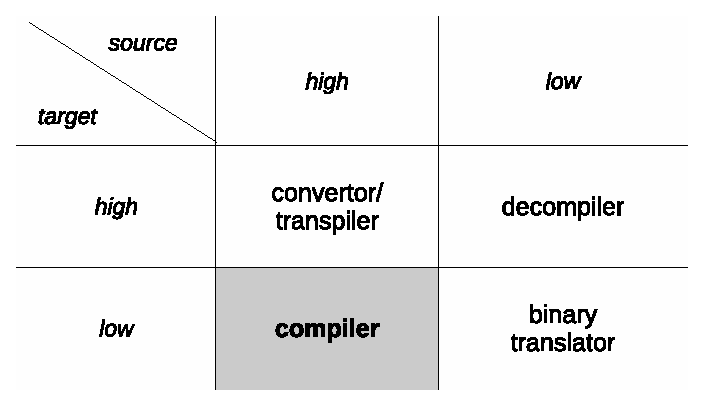
\includegraphics[scale=0.7]{images/01-05.eps}
\end{figure}

There is a somewhat common knowledge that among all these subspecies compilers are the most challenging to implement. While
we generally agree, it's worth mentioning that the other kinds of translators are not pieces of cakes at all: for example,
it is expeccted from a decompiler or convertor to properly utilize the abstractions of the target language, to produce a
human-readable maintanable results, etc.

\section{Environments and Cross-Compilation}

Programs are rarely work in isolation; as a rule they rely on a certain environment: operation system, system- and user-level
libraries, etc. Since compiler is a program itself, it also requires a certain environment, called \emph{compilation environment}.
On the other hand, the environment for which compiler generates its output is called \emph{target environment}. Usually that two
coinside~--- for example, out \lama compiler works under Linux on x86 processor, and generates programs which work
under Linux on x86.

However, in general case, compilation environment can be different from the target one. In this case the compiler is called
\emph{cross-compiler}. For example, we could rewrite our \lama compiler into a cross-one, which, still running on x86,
would generate code for ARM. 

A typical scenario for cross-compilation is \emph{bootstrapping} (see below) or the development of embedded systems when
the target platform is not enough performant/well-equipped to support the execution of a compiler.

\section{Bootstrapping}

An interesting (and practically important) operation involving compilers is their \emph{bootstrapping}. This term denotes the
implementation of a compiler in its own source languages (i.e. when implementation language coinsides with the source one).
The term itself originates from an idiom describing a process of pulling oneself up by the hooks on the back of their own
boots.

\begin{figure}[h]
  \centering
  \includegraphics[scale=0.2]{images/bootstrapping.png}
\end{figure}

The bootstrapping of a compiler for a new language (for which no compiler yet exists) is compised of its implementation
in some other language and then rewriting it in this new language using just written compiler. For example, in such a way the \lama compiler was
acquired (\textbf{not really yet}): initially it was implemented in \textsc{OCaml} and then reimplemented in
\lama itself.

If some compiler for the language of interest already exists, but works on some other platform, then it is possible for
implement a \emph{cross-compiler} which works on that platform but generates code for the platform of interest. Then
this compiler can be compiled by itself~--- this is the conventional way, for example, to port \textsc{GCC} compilers
to other platforms.

Finally, if nothing useful exists beside the assembler for the platform of interest, then this assembler itself can be
used to implement a small subset of the desirable language; then this subset can be used to implement a wider subset, and so on.
This is how modern compiler/language zoo was built historically.

Compiler bootstrapping is an ideologically important step: first, it assesses the expressivenes of the language; second, ir witnesses the
maturity of the compiler, since for a new language its compiler, as a rule, is the first large and complex program.

\section{Complete vs. Partial Correctness}

Compiler (as any other translator) has to syntactically transform a program in one language into a program in another, preserving its semantics.
In practice, however there are some subtleties.

Let us have a program $p$. We denote by

\[
x\xrightarrow{\displaystyle{p}} y
\]

the fact that $p$ on input $x$ terminates with the output $y$ (as we know, there may be two other outcomes: $p$ crashes on input $x$ or
$p$ loops forever on input $x$). 

Let us have a compiler, let $source$ be some source program, and let $target$ be a target program after the compilation.
We will say, that a compiler is \emph{complete correct}, iff for arbitrary $source$-$target$ pair and arbitrary
input-output pairs $x$ and $y$

\[
x\xrightarrow{\displaystyle{source}}y \Longleftrightarrow x\xrightarrow{\displaystyle{target}}y
\]

In other words, the behaviour of the source and compiled programs is indistinguishable: on the same input both either
terminate with the same results, or crash/loop.

Let us have, however, the following simple program:

\begin{lstlisting}[language=cc]
   # include <stdio.h>

   static int d = 0;

   int main (int argc, char *argv[]) {
     int x;

     x = argc / d;
    
     return 255;
   }  
\end{lstlisting}

A brief analysis reveals that this program has to crash on each input. Indeed, the variable ``\lstinline[language=cc,basicstyle=\normalsize]|d|'' has initial value zero and cannot
be reassigned elsewhere (due to ``\lstinline[language=cc,basicstyle=\normalsize]|static|'' storage class), and division by zero gives a runtime error. We could, alternatively,
try to compile this program with ``\texttt{gcc -O0}'' command and see that it, indeed, crashes.

On the other hand, a more careful analysis shows that the value of the variable ``\lstinline[language=cc,basicstyle=\normalsize]|x|'', during the computation
of which the error occurs, actually is never used, so its computation can be completely omitted. And, indeed, if we compile this program with the command ``\texttt{gcc -O3}'',
it terminates successfully with return code 255! This is because the option ``\texttt{-O3}'' turns on the optimizations, and one of those~--- \emph{dead code elimination}~---
does exactly what we envisioned.

Thus, we can see that in practice target programs not always completely equivalent to the source ones: they can deliver some results on inputs, for which the source
ones loop or crash. This property is called \emph{partial correctness}, and can be formally specified as for arbitrary $x$, $y$, $source$ and $target$

\[
x\xrightarrow{\displaystyle{source}}y \Longrightarrow x\xrightarrow{\displaystyle{target}}y
\]

This means, that when the source program terminates with a definite result, the target also does so; however, the target one can still deliver some output
values for inputs on which the source program is not defined. In other words, compilers are allowed to \emph{extend the domains} of programs they compile. The
majority of compilers (and other tools as well) are partially correct.

\section{Архитектура компиляторов}

С точки зрения архитектуры компиляторы в целом можно рассматривать как набор просмотров (passes), каждый из которых обрабатывает некоторое
промежуточное представление программы (intermediate representation). Конкретный набор как просмотров, так и форматов внутреннего представления
может отличаться от компилятора к компилятору. Среди наиболее употребимых внутренних представлений можно упомянуть абстрактное синтаксическое дерево
(abstract syntax tree), трехадресный код (three-address code), стековый код (stack machine code), статическую форму единственного присваивания (static
single assignment form, SSA) и другие. Некоторые из этих представлению будут нами использоваться при построении нашего компилятора, другие мы
оставим в стороне.

С точки зрения ассортимента просмотров в компиляторах как правило выделяют анализирующую и синтезирующую части. К анализирующей части относят,
прежде всего, синтаксический анализ и анализ типов (если в языке они есть). Существуют и другие задачи --- например, разрешение имен, работа с
областями видимости и т.д. Совокупность анализирующих просмотров часто объединяют понятием ``frontend'' (передняя часть компилятора).

К синтезирующей части относится деятельность по генерации машинного кода, например, выбор инструкций, распределение решистров, планирование и т.д.
Синтезирующие просмотры образуют так называемый ``backend'' компилятора, так сказать, его ``заднюю часть''.

Кроме этих двух компонент развитые компиляторы содержат набор оптимизирующий преобразований, который принято обозначать термином ``middle-end'',
так сказать, ``средняя часть'' компилятора. Количество просмотров в middle-end может быть достаточно велико, посколько существует более
десятка общеупотребимых оптимизирующих преобразований (некоторые указаны на слайде), котороые при компиляции могут повторяться.
<демонстрация>

\section{Компилятор \lama}

Теперь, когда мы обсудили, как устроены компиляторы вообще, давайте посмотрим, как устроен тот компилятор языка \lama, которым мы будем пользоваться
и который нам предстоит написать.

Наш компилятор устроен очень просто, горазда проще, чем компилятор GCC, который мы только что рассматривали для примера.

Исходный текстовой файл с программой на языке \lama поступает на вход синтаксического анализатора, который строит первое промежуточное
представление, называемое абстрактным синтаксическим деревом, или деревом абстрактного синтаксиса. Дерево абстрактного синтаксиса
является важнейшей формой представления программ, которая повсеместно используется не только для трансляции, но и для широкого
класса других языковых инструментов.

Следующей интересной компонентой, которая не всегда присутствует в промышленных компиляторх, является интерпретатор исходного языка.
Более подробно об интерпретаторах вообще мы поговорим позднее, пока же нам достатчно знать, что интерпретатор исполняет исходную программу,
в данном случае представленную в виде абстрактного синтаксического дерева, в соответствии с семантикой языка, на котором она написана.
Наличие интерпретатора в инфраструктуре \lama играет весьма важную как технологическую, так и дидактическую роль. Прежде всего,
реализация интерпретатора позволяет усвоить тот метод формального описания семантики языка программирования, которым мы будем пользоваться,
а именно~--- операционную семантику большого шага. Далее, наличие интерпретатора позволяет на ранних стадиях обнаруживать и исправлять
ошибки в синтаксическом анализаторе. Как мы увидим дальше, реализовать интерпретатор~--- относительно простая задача, и возможность
выполнить программу на ранних стадиях трансляции оказывается весьма полезной.

Следующей компонентой нашего компилятора является компилятор дерева абстрактного синтаксиса в код для стековой машины.
Эта машина напоминает упрощенную модель настоящего аппаратного процессора, поэтому, с одной стороны, для того, чтобы
сгенерировать код для этой машины, нужно решить похожие задачи, а с другой --- эти задачи решаются немного проще, чем
для настоящего процессора. Сгенерированный код для стековой машины можно исполнить на интерпретаторе стековой машины.
Так же как и в случае интепретатора исходного языка, возможность исполнить стековый код позволяет изолированно
отлаживать стековый компилятор.

Наконец, последней компонентой является собственно компилятор для x86, который преобразует стековый код в
программу на языке целевого ассемблера. После того, как эта программа порождена, она поступает на
вход инфраструктуре GCC, где проходит все остальные необходимые этапы до получения исполняемого модуля.

<демонстрация>

Таким образом, с точки зрения архитектуры, синтаксический анализатор относится к стадии анализа, а компиляторы
стековой машины и x86 --- к стадии синтеза.

\end{document}

